

\newpage
\section{Nonlinear FEM}
\label{s:Finite Element Modeling}

In this chapter the theory of FEM will be laid out.
The finite element method is a numerical technique used to obtain approximate solution to partial differential equations (PDEs) that represent physical problems. There are several techniques to obtain the approximate solution of PDEs. Some of the popular methods are:
\begin{enumerate}
\item Finite Difference Method (FDM)
\item Finite Volume Method (FVM)
\item Finite Element Method (FEM)
\item Boundary Element Method (BEM)
\item Spectral Method
\item Perturbation Method
\end{enumerate}
The main advantage of FEM consists of being able to deal with complex boundaries.
\subsection{Introduction to FEM}
The main steps of the solution process are indicated in the following picture
\begin{figure}[h]
\centering
  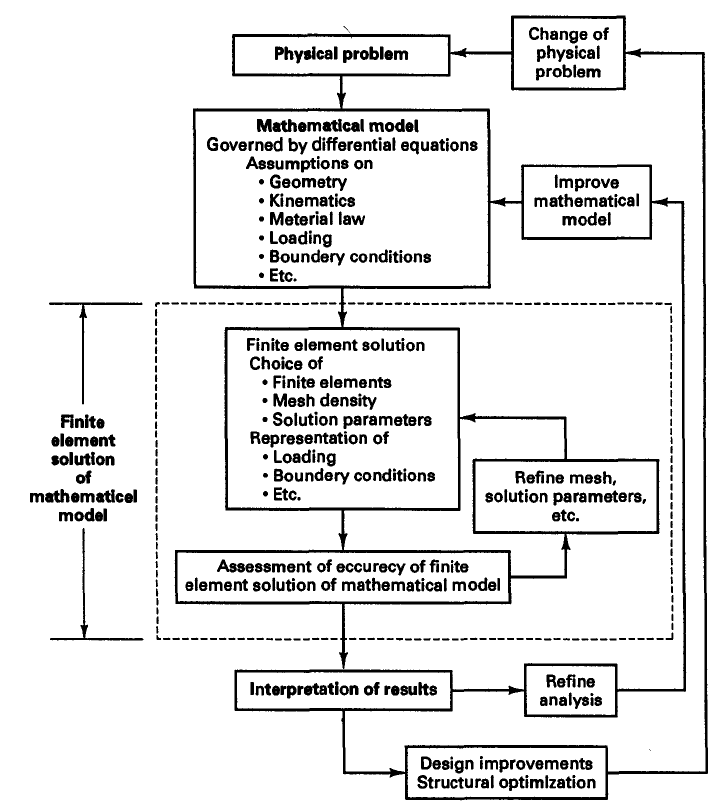
\includegraphics[height=12cm]{img/procedure.png}
   \caption{FEM process workflow.}
 \label{fgr:graft}
\end{figure}
In a first pre-processing phase you describe the problem: simplify a real engineering problem into a problem that can be solved by FEA. Then you discretized/mesh the solid, define material properties, apply boundary conditions.
Then you choose the processing conditions: approximate functions, formulate linear equations, and solve equations.
Finally, in the post-processing you obtain, visualize and explain the results.
\begin{enumerate}
\item Problem Formulation\\
The formulation of the specific governing the response of a system under specific loads and constraints at its boundaries is usually provided in the form of a differential equation. The differential equation is known as the \textit{strong form} of the problem and it includes
\begin{itemize}
\item Conservation of mass, momentum, energy
\item A measure of deformation, often called a strain-dispacement equation
\item A constitutive equation, which describes material behavior and relates stress to a measure of deformation
\end{itemize}
The following set of equations are a simple example:
\begin{align}
&\textrm{Equilibrium Equations:} &f(x)&=R+\frac{aL+ax}{2}(L-x)\\
&\textrm{Constitutive Requirements:}& \sigma&=E\epsilon\\
&\textrm{Kinematics Relationships:}& \epsilon&=\frac{du}{dx}
\end{align}
\item Discretization/Meshing\\
The continuum is discretized using a mesh of finite elements. These elements are connected at nodes located on the element boundaries.
\item Interpolation -The Shape Functions\\
The state of deformation, stresses, etc. in each element is approximated by a the set of corresponding values in the nodes; these nodal values are the basic unknowns of the MFE. Values between nodes, have to therefore result via interpolation.
\item 
\end{enumerate}


Three main methods exist when dealing with a FEM problem approximation: direct, variational and weighted residual method.
The direct approach is related to the “direct stiffness method” of structural analysis and is used for the analysis of discrete systems. For continuous and more complex  however, we have to use the other methods.
Continuous systems describe the physical behavior as a collection of infinitesimal material points(continuum).
Instead of enforcing equilibrium on the discrete system components, differential elements are used.
This results in a set of differential equations called strong form with the accompanying boundary conditions (essential and natural). 
These systems can be «discretized» and thus converted to discrete systems and be solved as in the direct solution.

The solution requires the following steps:
\begin{enumerate}
\item Discretization/idealization of the system into finite elements
\item Equilibrium relations with the element stiffness matrix
\item Determination of the stiffness properties
\item Build system of global algebraic equations
\item Determination of boundary conditions
\item Solve sequence: evaluation of degrees of freedom and response of each element 
\end{enumerate}

However in this differential approach the analytical solution is to difficult to evaluate because of complex geometries, loadings and boundary conditions.
Thus, instead of trying to solve the problem analytically, we would like to do it in an approximate, i.e., numerical way.
To this end, let us first consider what are the possible ways in which the system is allowed to deform. However in order to do it correctly we must check which are the kinematically admissible ways for the system to deform from a state $u(x)$ to a state $u(x)+\delta u(x)$. This is the case if:
\begin{enumerate}
\item $u(x)$ and $u(x)+\delta u(x)$: are continuous over the domain, \textit{i.e.} $u(x)  \in C_o \textrm{in} x \in [0, L]$
\item satisfy exactly the displacement BC, \textit{i.e.} $u(0)=0.$
\end{enumerate}

\begin{figure}[h]
\centering
  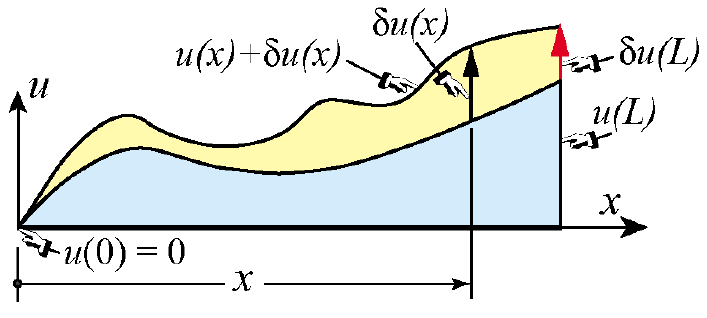
\includegraphics[height=5cm]{img/kinematic.png}
   \caption{Admissible displacements of $\delta u(x)$.}
 \label{fgr:graft}
\end{figure}
\subsubsection{Principle of Virtual Work}
The true deformation $u^*(x)$ is the one satisfying the principle of virtual work. The virtual work of a system of equilibrium forces vanishes when compatible virtual displacements $\delta u(x)$ are imposed:
\begin{equation}
\underbrace{	\int_{\Omega}\underline{\underline{\delta\epsilon}}:\underline{\underline{\sigma}} d\Omega
\rule[-12pt]{0pt}{5pt}}_{\mbox{Internal work}}
=
\underbrace{	\int_{\Omega}\delta u^{T} \cdot f^{B}d\Omega \rule[-12pt]{0pt}{5pt}}_{\mbox{Body forces (gravity)}}
+ 
\underbrace{	\int_{\Gamma}\delta u^{T} \cdot f^{S}d\Omega \rule[-12pt]{0pt}{5pt}}_{\mbox{Surface reactions}}
+ 
\underbrace{	\sum_{i}\delta u \cdot R_{C}^{i}			\rule[-12pt]{0pt}{5pt}}_{\mbox{Point loads}}
\end{equation}

With $\delta \vec{u}$ as Virtual Displacement must satisfy $ \vec{u}_r$ on $\Gamma_u$ and $\boldsymbol{\sigma}$ stress tensor and $\boldsymbol{\delta \epsilon}$ which is a function $\delta \vec{u}$.  
For elastic systems subject to conservative forces (which is the case of systems we are dealing with), the principle of Virtual Work is equivalent to principle of minimum total potential energy (MPE).
The MPE principle states that the actual displacement solution u*(x), out of possible trial solutions, that satisfies the governing equations is the one which renders the Total Potential Energy functional $\Pi$ stationary:
\begin{equation}
\delta \Pi = \delta U - \delta W=0 if u0u^*
\end{equation}
With U being internal energy (strain energy) and W external work.
If we assume $R^i_C$ is integrated into $\boldsymbol{f}^{\Gamma}$ it's equal to zero.

Given:
\begin{align*}
\boldsymbol{u}		&=\boldsymbol{H\hat{u}} & \boldsymbol{\delta u }	&=\boldsymbol{H\delta\hat{u}} & \boldsymbol{\sigma=C:\epsilon} \\
\boldsymbol{\epsilon}&=\boldsymbol{B\hat{u}} & \boldsymbol{\delta \epsilon}	&=\boldsymbol{B\delta\hat{u}=\delta\hat{u}^T B^T}
\end{align*}

Into the equation gives:
\begin{equation}
\int_{\Omega}\delta \boldsymbol{\hat{u}}^T\boldsymbol{B^TCB}\boldsymbol{\hat{u}} d \Omega
=
\int_{\Omega}\delta \boldsymbol{\hat{u}^{T}  H^{B} f^B } d\Omega 
+ 
\int_{\Gamma}\delta \boldsymbol{\hat{u}^{T}  H^{B} f^{\Gamma} } d\Gamma
\end{equation}

Arbitrary simplification of $\delta \textbf{u}$.
\begin{equation}
\underbrace{	\int_{\Omega} \boldsymbol{B^TCB}\boldsymbol{\hat{u}} d \Omega \rule[-12pt]{0pt}{5pt}}_{\mbox{\textbf{K} Stiffness matrix}}
=
\underbrace{	\int_{\Omega}\boldsymbol{H^{B} f^B } d\Omega \rule[-12pt]{0pt}{5pt}}_{\mbox{$\boldsymbol{F}^T$ Body force vector}}
+ 
\underbrace{	\int_{\Gamma} \boldsymbol{ H^{B} f^{\Gamma} } d\Gamma \rule[-12pt]{0pt}{5pt}}_{\mbox{$\boldsymbol{F}^S$ Body force vector}}
\end{equation}

Thus with the following:
\begin{align*}
\boldsymbol{K}&=\int_{\Omega} \boldsymbol{B^TCB}\boldsymbol{\hat{u}} d \Omega &	\boldsymbol{F}^B&=\int_{\Omega}\boldsymbol{H^{B} f^B } d\Omega & \boldsymbol{F}^S&=\int_{\Gamma} \boldsymbol{ H^{B} f^{\Gamma} } d\Gamma
\end{align*}
Yields:
\begin{equation}
\boldsymbol{K \hat{u}= F^B + F^S + \sum_{i} R_{C}^{i}= F}
\end{equation}


Discretized FEM equations:
\begin{equation}
\boldsymbol{K^{el} \hat{u}^{el}= F^{el}}
\end{equation}
These integrals must be computed in each element. This is mostly done numerically. Therefore elements have so-called "integration points"
\begin{equation}
\int f(\vec{x})d\vec{x}=\sum_{i=1}^{N_i}w_if_i
\end{equation}

\subsubsection{Weighted Residuals Method}
Weighted residual method (WRM) is a class of method used to obtain the approximate solution
to the differential equations of the form. It starts with an estimate of the the solution and demand that its weighted average error is minimized

\begin{equation}
\label{eq: diff}
\mathscr{L}(\phi) +f=0 \quad \textrm{in} \quad D
\end{equation}
It involves two major steps. In the first step, we assume an approximate solution
based on the general behavior of the dependent variable. It is selected to satisfy the boundary conditions for f. The assumed solution is then substituted in the differential equation. Since the assumed solution is only approximate, it does not satisfy the differential equation resulting in an error or what we call a residual. The residual is then made to vanish in some average sense over the entire solution domain. This procedure results in a system of algebraic equations. The second step is to solve the system of equations resulting from the first step subject to the prescribed boundary condition to yield the approximate solution sought.
Let $\psi(x) \approx \phi(x)$  be an approximation of the differential equation \ref{eq: diff}. When this is done it is unlikely that the equation is satisfied, thus $R(x)$ is a measure of error called \textit{residual}.
\begin{equation}
\label{eq: sub}
\mathscr{L}(\psi) +f=R
\end{equation}
If the equation \ref{eq: diff} is multiplied by an arbitrary \textit{weight function} and integrated over the domain $D$
\begin{equation}
\int_D w[\mathscr{L}(\phi) +f]dD=0 
\end{equation}
The equations are equivalent. Now, substituting for $\psi$ yields:
\begin{equation}
\label{eq: eq}
\int_D w(x)[\mathscr{L}(\psi) +f]dD=\int_D w(x)R(x) +f]dD \neq 0 
\end{equation}
The integral in \ref{eq: eq} gives the weighted average of the residual over the solution domain. In weighted residual method we force this integral to vanish over the solution domain. That is,
\begin{equation}
\int_D w(x)R(x)dD=0 
\end{equation}
In the form of a generalized Fourier series the function can be approximated as following:
\begin{equation}
\psi(x)=\sum_{i=1}^nc_iN_i(x)=c_1N_1(x)+c_2N_2(x)+...+c_nN_n(x)
\end{equation}
In vector form
\begin{equation}
\boldsymbol{\psi(x)=C^TN^T=(NC)^T=NC}
\end{equation}
Where \textbf{N} is the row vector 
\begin{equation}
\boldsymbol{N}=
\begin{matrix}
[ N_1	& N_2 & ... & N_n ]
\end{matrix}
\end{equation}
And \textbf{C} is the column vector 
\begin{equation}
\boldsymbol{C}=\left[
\begin{matrix}
C _1	\\ C_2 \\ ... \\ C_n 
\end{matrix} \right]
\end{equation}
Here $ci$’s are unknown coefficients called\textit{ fitting coefficients} and $n$ is the number of fitting coefficients. $N_i(x)$’s are assumed to be linearly independent functions of x and are called \textit{trial functions}.
The trial functions can be polynomials, trigonometric functions etc. The trial functions are usually chosen in such a way that the assumed function $\psi(x)$ satisfies the global boundary conditions for $\phi (x)$, although this not strictly necessary and certainly not always possible.

Polynomial Approximation. One of the simplest choices for a trial function is a polynomial, for a one-dimensional problem which can be obtained by taking $N_i(x) = x^i$. The result is
\begin{equation}
\psi(x)= \sum_{i=0}^nc_ix^i=c_0+c_1x+...+c_nx^n
\end{equation}
This produces a smooth solution, but it suffers the same limitations as Lagrange interpolation. A particularly significant flaw is that this choice need not converge to $\phi(x)$ as $n$ increases.
With the selection of $\psi(x)$ as the series expansion (4.6), it is evident that the residual $R$ depends on the unknown parameters $c_i$’s in the expansion:
\begin{equation}
R=R(x;C)
\end{equation}
If the number of trial functions n is sufficiently large, then in principle, the unknown parameters $ci$’s can be chosen so that the residual $R$ is small over the domain.
Weight functions. In general the weight function $w(x)$ may be written as
\begin{equation}
w(x)= \sum_{i=0}^na_iw_i=a_1w_1+a_2w_2+...+a_nw_n=\boldsymbol{aw}
\end{equation}
Where \textbf{a} and \textbf{w} are respectively the row  and the column vectors
\begin{equation}
\boldsymbol{a}=
\begin{matrix}
[ a_1	& a_2 & ... & a_n ],
\end{matrix} 
\quad 
\boldsymbol{w}=\left[
\begin{matrix}
w _1	\\ w_2 \\ ... \\ w_n 
\end{matrix} \right]
\end{equation}
Here $wi$’s are known functions of x and ai’s are constant parameters. Substituting $w(x) = \boldsymbol{aw}$ in
the weighted residual equation (4.5) to yield
\begin{equation}
\boldsymbol{a\int_Dw}RdD=0
\end{equation}
Since \textbf{a} is a constant vector, we have
\begin{equation}
\boldsymbol{\int_Dw}RdD=0
\end{equation}or
\begin{align}
\boldsymbol{\int_Dw_1}RdD=0\\
...\\
\boldsymbol{\int_Dw_n}RdD=0
\end{align}
Now we have $n$ equations to determine unknown coefficients $ci$’s. Finally, inserting $\psi = \boldsymbol{NC}$ in
equation \ref{eq: sub} yields
\begin{equation}
R=\mathscr{L}(\boldsymbol{NC})+f=\mathscr{L}\boldsymbol{(N)C}+f
\end{equation}
and hence the 
\begin{equation}
\left[\int_D \boldsymbol{w}\mathscr{L}(\boldsymbol{N})dD\right]\boldsymbol{C}=-\int_D\boldsymbol{w}fdD
\end{equation}
Introduction matrix \textbf{K} and \textbf{f }as
\begin{equation}
\boldsymbol{K}=\int_D \boldsymbol{w}\mathscr{L}(\boldsymbol{N})dD, \quad \boldsymbol{f}=-\int_D\boldsymbol{w}fdD
\end{equation}

allows us to write the equation in compact form 
\begin{equation}
\boldsymbol{KC=f}
\end{equation}
The system of equations can be solved for n unknown coefficients $ci$’s provided that a suitable weight function $w$ is selected.
With regards to the selection of weight function, we have several choices. Hence, depending
upon nature of weight function, we have different types of weighted residual methods. Some of
the standard methods are:
\begin{enumerate}
\item Point Collocation Method
\item  Subdomain Collocation Method
\item  Least Square Method
\item  Galerkin Method
\end{enumerate}

\paragraph{Galerkin Method}
In Galerkin version of weighted residual method, the weight functions are chosen to be the trial
functions themselves. This is the method we usually used for developing finite element equations
for field problems. So, in Galerkin method we set
\begin{equation}
w_i=N_i \quad (i=1,2,...,n)
\end{equation}
The unknown coefficients in the approximate solution are determined by setting the integral
over D of the weighted residual to zero. For one-dimensional problem in the interval [a,b], this
procedure will results
\begin{equation}
\int_a^bw_iR(x)dx=\int_a^bN_iR(x)dx=0
\end{equation}Following points about Galerkin method may be noted:
• Galerkin method produces symmetric positive definite coefficient matrix if the differential
operator is self-adjoint.
• Galerkin method requires less computational effort compared to the least square method.
\subsubsection{Variational Method}
In this approach the physical problem is restated using the aforementioned principle of minimum potential energy. This variational form is also know as the weak form and it is widely used for deriving finite element equations whenever classical variational statement is available for the given problem. For approximate solutions, a larger class of trial solutions $u(x)$ can be employed than in the differential formulation; for example, the trial functions do not need to satisfy the natural BC because these are implicitly contained in the functional. The approximation is based on the minimization of the functional.
The major drawback of this approach is that it's not useful for nonlinear problems . 
The Rayleigh-Ritz method is an approximate method based on the variational formulation.
If you consider a PDE with variational structure the variational form of 
\begin{equation}
I(u)=\int_{\Omega}[\frac{k}{2}\left(\frac{\partial u}{\partial x_1}\right)^2+\frac{k}{2}\left(\frac{\partial u}{\partial x_2}\right)^2 +fu]d\Omega
\end{equation}
\paragraph{Rayleigh-Ritz Method}
Rayleigh–Ritz method replaces the trial functions into the functional (variational) form of the PDE. It's advantageous since less differentiability is required and the natural boundary conditions are already in the function. Hence, there is no need for the trial functions to satisfy them.
\begin{equation}
\hat{u}=\sum_{i=1}^nw_if_i\cong u(x)
\end{equation}
Thus the functions $f_i$ only need to be differentiable once and it only needs to satisfy $u_0=0$



\subsubsection{Isoparameteric Continuum Elements}
In general, we would like to be able to represent any element in a standardized manner –introducing a transformation between a set of standardized (natural) coordinates and the real (global) coordinates
Different schemes exist for establishing such transformations: isoparametric representations (same nodes for both geometry and displacement representation)
Displacement fields as well as the geometrical representation of the finite elements are approximated using the same approximating functions –shape functions. This transformation allows us to refer to similar elements (eg. truss, beams, 2D elements, in a standard manner, using the natural coordinates (r,s), without every time referring to the specific global coordinate system (x,y).
Isoparametric elements can be one-, two-or three-dimensional:

The principle is to assure that the value of the shape function hiis equal to one in node iand equals zero in other nodes.

In order to establish the stiffness matrixes we must differentiate the displacements with respect to the coordinates (x, y, z). Since the shape functions are usually defined in natural coordinates we must introduce the necessary coordinate transformation between natural and global or local coordinate system. For example in the 3D domain we can express the derivative of a function which is expressed in terms of coordinates (x,y,z), with respect to an other set of coordinates (r,s,t) as:


\paragraph{Shape Function}
Shape functions will be defined as interpolation functions which relate the variables in the finite element with their values in the element nodes. The latter are obtained through solving the problem using finite element procedures.
Regardless of the dimension of the element used, we have to bear in mind that Shape Functions need to satisfy the following constraints:
\subsection{Continuum mechanics}
In case of linear deformation the reference and current configurations coincide.
For large deformations the difference is important. The reference configuration is independent of time, this means a reference point will always correspond to a material particle, hence \textit{material configuration}. This is also denoted as \textit{Lagrangian Configuration} as it is from the Lagrangian viewpoint. On the other hand the point in the current configuration do not correspond to the material points, but to the points in space. This is denoted \textit{spatial configuration} and corresponds the a material flow through a fixed domain as postulated by the Eulerian viewpoint, hence \textit{Eulerian Configuration}.
The differences between Lagrangian and Eulerian meshes are most clearly seen in terms of the behavior of the nodes. If the mesh is Eulerian, the Eulerian coordinates of nodes are fixed, i.e. the nodes are coincident with spatial points. If the mesh is Lagrangian, the Lagrangian material coordinates X of nodes are time invariant, i.e. the nodes are coincident with material points.
\begin{figure}
\centering
  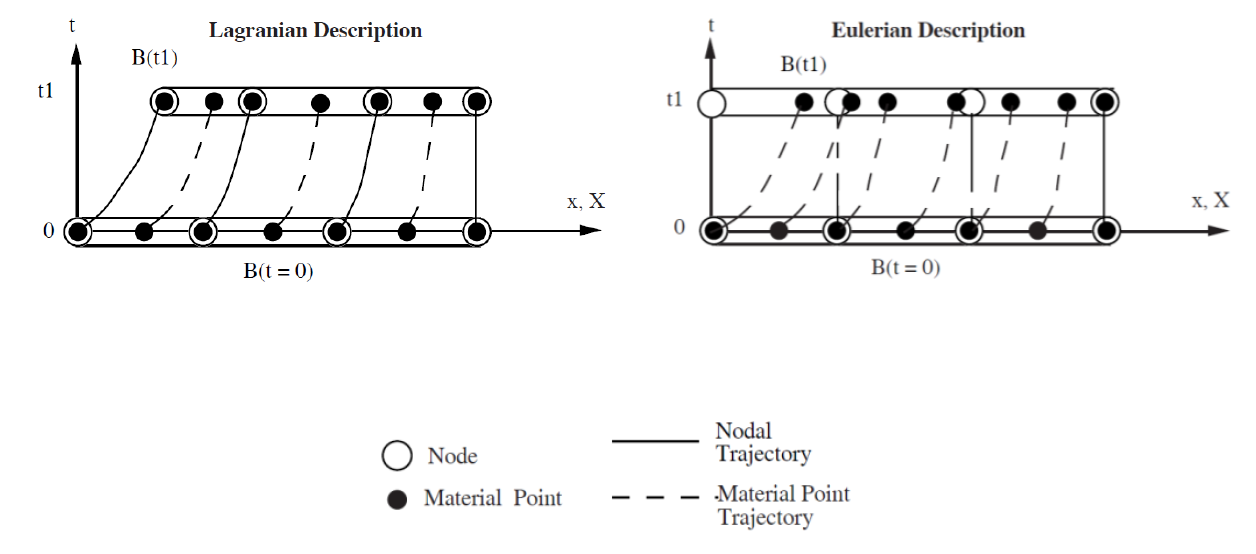
\includegraphics[height=4cm]{img/ale.png}
   \caption{Space time depiction of a one dimensional Lagrangian, Eulerian and ALE (arbitrary Lagrange Eulerian) element.}
 \label{fgr:graft}
\end{figure}
In the Eulerian mesh, the nodal trajectories are vertical lines and material points pass across element interfaces.
In the Lagrangian mesh, nodal trajectories are coincident with material point trajectories, and no material passes between elements. Furthermore,
element quadrature points remain coincident with material points in Lagrangian meshes, whereas in Eulerian meshes the material point at a given
quadrature point changes with time. We will see later that this complicates the treatment of materials in which the stress is history-dependent. In Lagrangian meshes, since the material points remain coincident with mesh points, the elements deform with the material. Therefore, elements in a
Lagrangian mesh can become severely distorted. This effect is apparent in a onedimensional problem only in the element lengths: in Eulerian meshes, the
element length are constant in time, whereas in Lagrangian meshes, element lengths change with time. In multi-dimensional problems, these effects
are far more severe, and elements can get very distorted. Since element accuracy degrades with distortion, the magnitude of deformation that can be
simulated with a Lagrangian mesh is limited. Eulerian elements, on the other hand, are unchanged by the deformation of the material, so no degradation in accuracy occurs because of material deformation.
The comparative advantages of Eulerian and Lagrangian meshes can be seen even in this simple one-dimensional example. Since the nodes are
coincident with material points in the Lagrangian mesh, boundary nodes remain on the boundary throughout the evolution of the problem. This
simplifies the imposition of boundary conditions in Lagrangian meshes.
In Eulerian meshes, on the other hand, boundary nodes do not remain coincident with the boundary. Therefore, boundary conditions must be imposed at points which are not nodes, and as we shall see later, this engenders significant complications in multi-dimensional problems. Similarly, if a node is placed on an interface between two materials, it remains on the interface in a Lagrangian mesh, but not in an Eulerian mesh.

\begin{figure}
\centering
  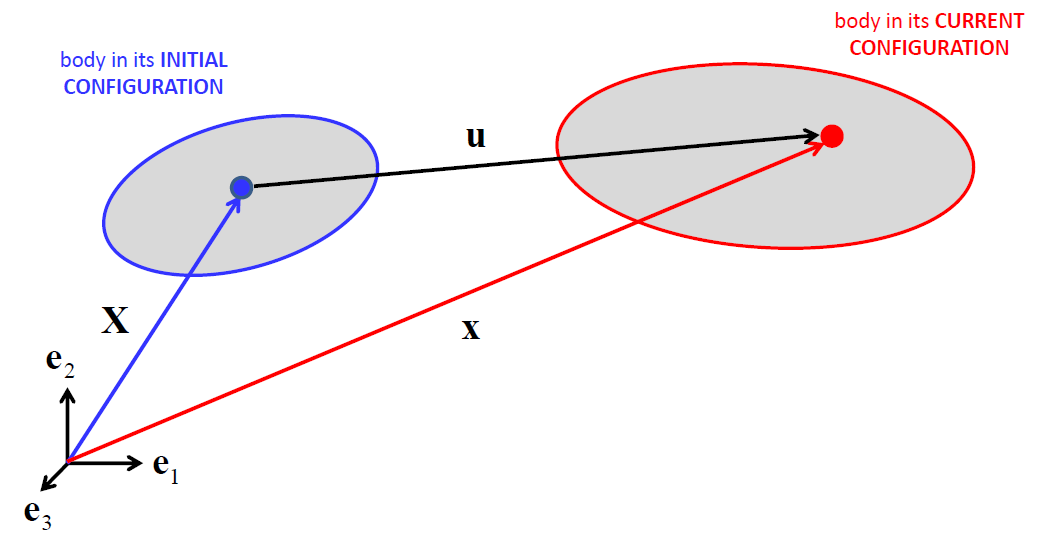
\includegraphics[height=6cm]{img/Def.png}
   \caption{adaptive mesh generation}
 \label{fgr:graft}
\end{figure}
Displacement:
\begin{equation}
u=x-X
\end{equation}

\begin{align}
&\textrm{Reference configuration:}& u(X,t)&=\phi(X,t)-X \\
&\textrm{Current configuration:}& u(x,t)&=x-\phi^{-1}(x,t)
\end{align}

Velocity:
\begin{align}
&\textrm{Reference:}	&(X,t)&=\frac{\partial u(X,t)}{\partial t}=\frac{\partial \phi (X,t)}{\partial t} -  \cancelto{0}{\frac{\partial X}{\partial t}}=\frac{\partial\phi (X,t)}{\partial t}=\dot{u} \\
&\textrm{Current:}		&(x,t)&=\frac{\partial (x-X)}{\partial t}=\frac{\partial x}{\partial t}
\end{align}

Acceleration:
\begin{align}
&\textrm{Reference:}	&a(X,t)&=\frac{\partial v(X,t)}{\partial t}=\frac{\partial^2 \phi (X,t)}{\partial t^2} =\dot{v} \\
&\textrm{Current:}		&(x,t)&=\frac{\partial (x-X)}{\partial t}=\frac{\partial x}{\partial t}
\end{align}

\begin{equation}
dx=FdX
\end{equation}

Material Time Derivative:

\begin{equation}
a(\underline{v},t)=\frac{D}{Dt}(\underline{v})=\frac{\partial\underline{v}}{\partial t}+\nabla\underline{v}\cdot \underline{v}
\end{equation}

\begin{equation}
\frac{D()}{Dt}=\frac{\partial}{\partial t}()+\nabla ()\cdot \underline{v}
\end{equation}

Deformation Gradient:
\begin{equation}
\boldsymbol{F}=\frac{\partial x}{\partial X}=\frac{\partial x_i}{\partial X_j}=\begin{matrix}
 -1 & 3 \\
  2 & -4
\end{matrix}
\end{equation}

\subsubsection{Stress Measures}
The definition of stress measures depends on the selected configuration.
Thus different stress measures can be defined. The most common stress definitions are:
\begin{itemize}
\item Nominal stress (engineering stress)
\item True stress (Cauchy stress)
\item Corotational stress
\item 1st Piola Kirchhoff stress (PK1)
\item 2nd Piola Kirchhoff stress (PK2)
\end{itemize}


\paragraph{Generalized Principle of Virtual Work}
\begin{align*}
&\textrm{Conservation of Momentum:} & \boldsymbol{\nabla\sigma+f}^{B}	&=0 			&\textrm{on} \quad \Omega
\\
&\textrm{Force BC:} 				& \boldsymbol{\sigma\cdot n	}		&=\boldsymbol{f}^{\Gamma} &\textrm{on} \quad \Gamma_{f}
\\
&\textrm{Displacement BC:}			& \boldsymbol{u}						&=\boldsymbol{u}^{\Gamma} &\textrm{on} \quad \Gamma_{u}
\\
&\textrm{Galerkin Approach:} & \int_{\Omega}(\nabla\underline{\underline{\sigma}}+\underline{f}^{B})\underline{\delta u}d\Omega&=0 
\\
& & \int_{\Gamma}(\underline{\underline{\sigma}}\cdot \underline{a}+\underline{f}^{M})\underline{\delta u}d\Gamma&=0 
\end{align*}
Choose $\underline{\delta u}$ such that $\underline{\delta u}=u^{\Gamma}$ on $\Gamma_{u}$. Essential BC's are embedded into the trial functions.

\begin{equation}
\int_{\Omega}\nabla\underline{\underline{\sigma}}\delta u d\Omega+ \int_{\Omega}f^B \delta u d\Omega - \int_{\Omega}\underline{\underline{\sigma}} \cdot \underline{n} \cdot \underline{\delta u} d\Gamma + \int_{\Gamma}\underline{f}^{B} \underline{\delta u} d\Omega = 0
\end{equation}

Product rule in 3D
\begin{equation}
\nabla (\underline{\underline{T}}\cdot \underline{v})= \nabla T \cdot \underline{v}+ T:\nabla v
\end{equation}
\subsubsection{Numerical Issues - Instability problems}

\subsection{Implicit/explicit FEM}



\begin{figure}[h]
\centering
  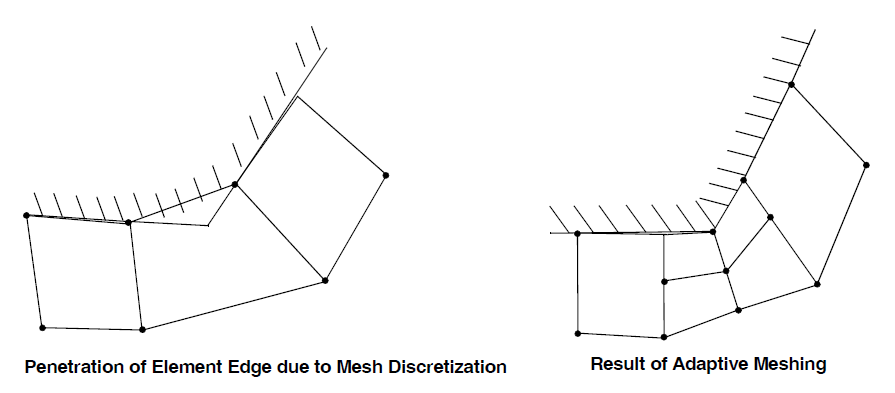
\includegraphics[height=4cm]{img/Adaptive.png}
   \caption{adaptive mesh generation}
 \label{fgr:graft}
\end{figure}

